\chapter{Pemrograman Dasar}
Tujuan pembelajaran pada pertemuan kedua antara lain:
\begin{enumerate}
\item
Mengenal Jenis Variabel Python
\item
Input dan output user
\item
Operator Dasar
\item
Perulangan
\item
Kondisi
\item
Mengatasi Error
\item
Try Except
\end{enumerate}
Tugas dengan cara dikumpulkan dengan pull request ke github dengan menggunakan latex pada repo yang dibuat oleh asisten IRC. Kode program dipisah dalam folder src NPM.py yang berisi praktek dari masing-masing tugas file terpisah sesuai nomor yang kemudian dipanggil menggunakan input listing ke dalam file latex penjelasan atau nomor pengerjaan. Masing masing soal bernilai 5 dengan total nilai 100.

\section{Teori}
Praktek teori penunjang yang dikerjakan :
\begin{enumerate}
\item
sebutkan jenis-jenis variabel dan jelaskan cara pemakaian variabel tersebut di kode Python
\item
tuliskan bagaimana kode untuk meminta input dari user dan tuliskan bagaimana melakukan output ke layar
\item
Tuliskan operator dasar aritmatika, tambah, kali, kurang bagi, dan 
bagaimana mengubah string ke integer dan integer ke string
\item
Tuliskan dan jelaskan sintak untuk perulangan, jenis-jenisnya contoh kode dan cara pakainya di python
\item
Tuliskan jelaskan cara pakai sintak untuk memilih kondisi, dan bagiamana contoh sintak kondisi di dalam kondisi.
\item
Tuliskan apa saja jenis error yang sering ditemui di python dalam mengerjakan sintak diatas. 
dan bagaimana cara mengatasinya
\item
Tuliskan dan jelaskan cara memakai Try Except.
\end{enumerate}

\section{Ketrampilan Pemrograman}
Buat program di python dengan ketentuan:
\begin{enumerate}
\item
Buatlah luaran huruf yang dirangkai dari tanda bintang, pagar atau plus dari NPM kita.
Tanda bintang untuk NPM mod 3=0, tanda pagar untuk NPM mod 3 =1, tanda plus untuk NPM mod3=2.
Contoh Output : 
\begin{verbatim}
*****    *** ******     *****    ****
*******  *** ***  **    *** **  *****
***  ******* ******     ***  **** ***
***    ***** ***        ***       ***
***     **** ***        ***       ***
\end{verbatim}
NPM sesuai dengan nomor NPM nya.
\item
Buatlah program hello word dengan input NPM yang disimpan dalam sebuah variabel string bernama \textbf{NPM} dan output sebanyak dua dijit belakang NPM, 
contoh NPM : 113040087 maka akan ada output sebanyak 87 dengan tulisan `Hallo, 113040087 apa kabar?'
\begin{verbatim}
Input : 113040087
Output : 
Halo, 113040087 apa kabar? 
Halo, 113040087 apa kabar?
Halo, 113040087 apa kabar?
Halo, 113040087 apa kabar?
Halo, 113040087 apa kabar?
Halo, 113040087 apa kabar?
Halo, 113040087 apa kabar?
Halo, 113040087 apa kabar?
.....87 kali...
\end{verbatim}
\item
Buatlah program hello word dengan input nama yang disimpan dalam sebuah variabel string bernama \textbf{NPM} dan beri luaran output berupa tiga karakter belakang dari NPM sebanyak penjumlahan tiga dijit tersebut, 
\begin{verbatim}
Input : 113040087
Output : Halo, Nama apa kabar? 
Halo, 087 apa kabar?
Halo, 087 apa kabar?
Halo, 087 apa kabar?
Halo, 087 apa kabar?
Halo, 087 apa kabar?
Halo, 087 apa kabar?
Halo, 087 apa kabar?
........15 kali(0+8+7).........
\end{verbatim}
\item
Buatlah program hello word dengan input nama yang disimpan dalam sebuah variabel string bernama \textbf{NPM} dan beri luaran output berupa digit ketiga dari belakang dari variabel NPM, 
\begin{verbatim}
Input : 113040087
Output :
Halo, 0 apa kabar?
\end{verbatim}
\item
\label{digitvar}
(untuk soal no \ref{digitvar} dan selanjutnya wajib menggunakan perulangan dan kondisi) buat program dengan mengisi variabel alfabet dengan nomor npm satu persatu berurut.
Contoh untuk NPM : 113040087 maka,
\begin{verbatim}
a = 1
b = 1
c = 3
e = 0
f = 4
g = 0
h = 0
i = 8
j = 7
\end{verbatim}
Lakukan print NPM lengkap anda menggunakan variabel diatas :

contoh : 113040087
\item
Dari soal no \ref{digitvar}, Lakukan penjumlahan dari seluruh variabel tersebut,
\item 
Dari soal no \ref{digitvar}, Lakukan perkalian dari seluruh variabel tersebut,
\item
Dari soal no \ref{digitvar}, Lakukan print secara vertikal dari NPM anda menggunakan variabel diatas. Contoh:
\begin{verbatim}
1
1
3
0
4
0
0
8
7
\end{verbatim}
\item
Dari soal no \ref{digitvar}, Lakukan print NPM anda tapi hanya dijit genap saja. Contoh:
\begin{verbatim}
48
\end{verbatim}
\item
Dari soal no \ref{digitvar}, Lakukan print NPM anda tapi hanya dijit ganjil saja. Contoh:
\begin{verbatim}
1137
\end{verbatim}
\item 
Dari soal no \ref{digitvar}, Lakukan print NPM anda tapi hanya dijit yang termasuk bilangan prima saja. Contoh:
\begin{verbatim}
37
\end{verbatim}
\end{enumerate}


\section{Ketrampilan Penanganan Error}
Bagian Penanganan error dari script python.
\begin{enumerate}
\item
Tuliskan peringatan error yang didapat dari mengerjakan praktek kedua ini, dan jelaskan cara penanganan error tersebut.
\item
Membuat file 2err.py dan mengisinya dengan script pengisian variabel sebagai string dan pengisian variabel sebagai interger. 
Kemudian jumlahkan antara variabel integer dan string dan tangkap jenis errornya, gunakan try except untuk menunjukkan error tersebut dengan
bahasa indonesia.
\end{enumerate}

\section{Jawaban Teori Chapter 2}
\begin{enumerate}
    \item Jenis Jenis Variabel dan Cara pemakaian Variabel tersebut di Python
    \par Variabel adalah lokasi memori yang dicadangkan untuk menyimpan nilai-nilai. Ini berarti bahwa ketika Anda membuat sebuah variabel Anda memesan beberapa ruang di memori. Variabel menyimpan data yang dilakukan selama program dieksekusi, yang natinya isi dari variabel tersebut dapat diubah oleh operasi - operasi tertentu pada program yang menggunakan variabel.
    \par
    Variabel dapat menyimpan berbagai macam tipe data. Di dalam pemrograman Python, variabel mempunyai sifat yang dinamis, artinya variabel Python tidak perlu didekralasikan tipe data tertentu dan variabel Python dapat diubah saat program dijalankan.
    \par
    \begin{figure}[!htbp]
    \centering 
    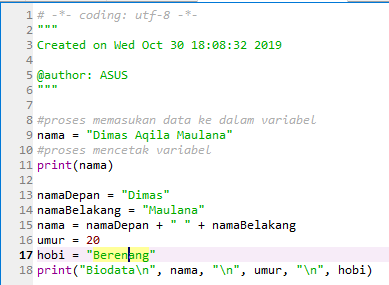
\includegraphics[scale=0.9]{figures/pemakaianvariabel.PNG} 
    \caption{Pemakaian Variabel di Python}
    \label{variabel}
    \end{figure}
    \item Input data user dan Output ke layar
    \par
    Cara menginputkan ke dalam python dengan cara membuat codingan seperti
    pada gambar\ref{inputoutput1}
    \begin{figure}[!htbp]
    \centering 
    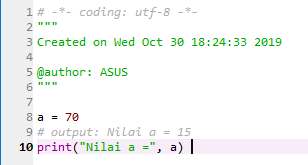
\includegraphics[scale=1.2]{figures/inputoutput1.PNG} 
    \caption{Cara menginputkan ke aplikasi Spyder}
    \label{inputoutput1}
    \end{figure}
    \par
    Setelah inputan sudah dimasukkan lalu akan ada output pada bagian kanan spyder seperti pada gambar\ref{inputoutput2}
        \begin{figure}[!htbp]
    \centering 
    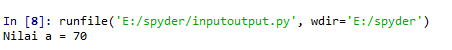
\includegraphics[scale=1.2]{figures/inputoutput2.PNG} 
    \caption{Output yang keluar}
    \label{inputoutput2}
    \end{figure}
    \item Operator dasar aritmatika dan mengubah string ke interger atau sebaliknya
    \par
    Operator dasar aritmatika ada 6 yaitu kali, tambah, bagi, kurang, sisa, dan pangkat pada gambar dibawah adalah kodingan aritmatika dasar dalam matematika \ref{aritmatika}
        \begin{figure}[!htbp]
    \centering 
    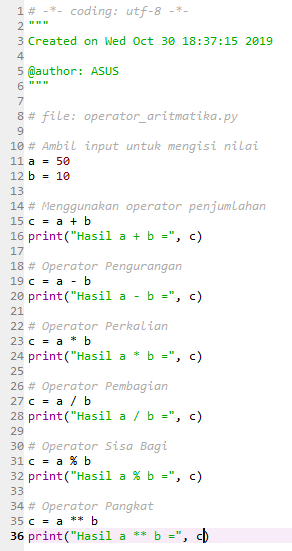
\includegraphics[scale=0.9]{figures/aritmatika.PNG} 
    \caption{Operasi Dasar Aritmatika}
    \label{aritmatika}
    \end{figure}
    \par
    Cara mengubah string ke integer dan integer ke string ada pada gambar berikut \ref{aritmatika2}
    \par
            \begin{figure}[!htbp]
    \centering 
    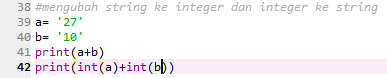
\includegraphics[scale=0.9]{figures/aritmatika2.PNG} 
    \caption{Mengubah integer ke string}
    \label{aritmatika2}
    \end{figure}
    \item Sintak sintak untuk perulangan, jenis jenisnya, contoh kode dan cara pakai di python
    \par
    Pengulangan adalah salah satu hal penting yang ada di bahasa pemrograman. Pengulangan digunakan misalnya untuk meng-update nama file yang cukup banyak jumlahnya, atau mengakses piksel satu persatu pada gambar.
    \par
    Dengan menggunakan while, kalian dapat membuat kondisi tertentu untuk menghentikan while. Biasanya while digunakan untuk melakukan looping yang tidak pasti contohnya seperti pada gambar \ref{perulangan1}
    \begin{figure}[!htbp]
    \centering 
    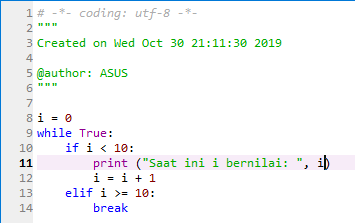
\includegraphics[scale=0.9]{figures/perulangan1.PNG} 
    \caption{Sintak Perulangan}
    \label{perulangan1}
    \end{figure}
    \par
    Pengulangan for biasa digunakan untuk pengulangan yang sudah jelas banyaknya. Misal, Anda ingin mengulang sebuah pengulangan sampai 10 kali atau mengeluarkan semua hasil query dari database di halaman HTML. Berikut ini adalah contoh kode untuk pengulangan for seperti pada kodingan dibawah.
    \par
    for i in range(0, 10):
    \par
    print i
    \par
    \item Cara pakai sintak untuk memilih kondisi,dan contohnya
    \par
    Berikut ini adalah contoh penggunaan if di Python terlihat pada gambar \ref{kondisi1}
    \begin{figure}[!htbp]
    \centering 
    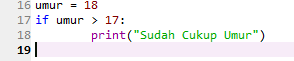
\includegraphics[scale=1.2]{figures/kondisi1.PNG} 
    \caption{Kondisi If}
    \label{kondisi1}
    \end{figure}
    \par
    Untuk memeriksa kondisi yang tidak memenuhi kondisi utama. Maka else digunakan untk menangani semua kondisi selain kondisi yang telah dituliskan. Berikut adalah contoh penggunaan else di dalam kondisional Python:
    \begin{figure}[!htbp]
    \centering 
    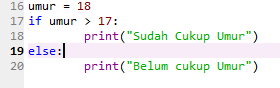
\includegraphics[scale=1.2]{figures/kondisi2.PNG} 
    \caption{Kondisi Else}
    \label{kondisi2}
    \end{figure}
    \par
    \item Jenis error yang sering ditemui dalam python dan cara menyelesaikannya
    \par
    Terjadi error pada sintak kondisi ketika akan cetak print tidak memakail tanda ("") karena yang dicetak print adalah variabel string, cara mengatasinya tinggal tambahkan sintak ("") setelah tulisan print. Contohnya print ("Umur anda 20 tahun")
    \item Cara memakai Try Except
    \par
    Dalam membuat suatu program pasti ada saja kode yang membuat program error saat di running. Salah satu cara menyelesaikannya dengan cara menggunakan statment try except seperti pada gambar \ref{tryexcept}
\begin{figure}[!htbp]
    \centering 
    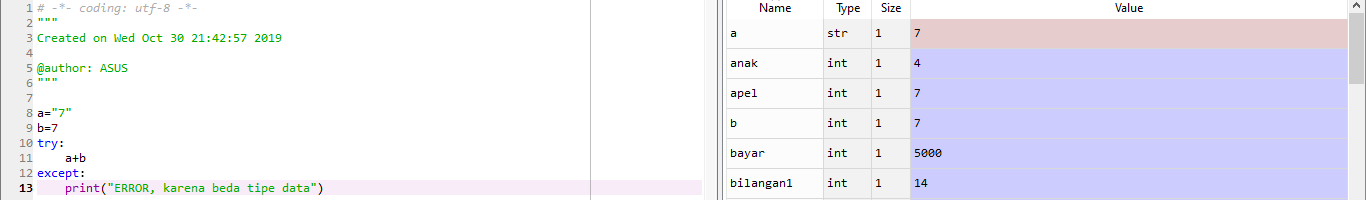
\includegraphics[scale=0.4]{figures/tryexcept.PNG} 
    \caption{Try Except}
    \label{tryexcept}
    \end{figure}
\end{enumerate}

